\documentclass{beamer}
\usepackage{beamerthemesplit}
\usepackage{wrapfig}
\usetheme{SPbGU}
\usepackage{pdfpages}
\usepackage{amsmath}
\usepackage{mathtools}
\usepackage{cmap} 
\usepackage[T2A]{fontenc} 
\usepackage[utf8]{inputenc}
\usepackage[english,russian]{babel}
\usepackage{indentfirst}
\usepackage{amsmath}
\usepackage{tikz}
\usepackage{multirow}
\usepackage[noend]{algpseudocode}
\usepackage{algorithm}
\usepackage{algorithmicx}
\usetikzlibrary{shapes,arrows}
\usepackage{fancyvrb}
\newtheorem{rutheorem}{Теорема}
\newtheorem{ruproof}{Доказательство}
\newtheorem{rudefinition}{Определение}
\newtheorem{rulemma}{Лемма}
\beamertemplatenavigationsymbolsempty

\title[]{Теория автоматов и формальных языков}
\subtitle[]{Введение}
\institute[]{
Санкт-Петербургский государственный электротехнический университет <<ЛЭТИ>>\\
}

\author[]{Екатерина Вербицкая}

\date{ сентября 2016г.}

\definecolor{orange}{RGB}{179,36,31}

\begin{document}
{
  \begin{frame}
    \titlepage
  \end{frame}
}


\begin{frame}[fragile]
  \transwipe[direction=90]
  \frametitle{Контекст: языки}
  \begin{itemize}
    \item Естественные 
    \begin{itemize}
      \item Русский, английский...
    \end{itemize}    
    \pause
    \item Искусственные
    \begin{itemize}
      \item Эсперанто, ложбан...
      \item Клингонский, эльфийский...
      \pause
      \item C++, Java, C\#, Haskell, OCaml, Perl, Coq, Agda...
    \end{itemize}
  \end{itemize}
\end{frame}
            

\begin{frame}[fragile]
  \transwipe[direction=90]
  \frametitle{Контекст: языковые процессоры}
  \begin{itemize}
    \item Текстовые редакторы
    \item Компиляторы, интерпретаторы, трансляторы
    \item Среды разработки
  \end{itemize}

  \begin{itemize}
    \item Все нуждаются в некотором формализованном представлении языка
  \end{itemize}
\end{frame}

\begin{frame}[fragile]
  \transwipe[direction=90]
  \frametitle{Язык программирования}
  \begin{itemize}
    \item Синтаксис --- правила построения программ из символов
    \item Семантика --- правила истолкования программ, определяющие их смысл
  \end{itemize}
\end{frame}


\begin{frame}[fragile]
  \transwipe[direction=90]
  \frametitle{Пример: язык арифметических выражений}
  \begin{itemize}
    \item Алфавит символов: цифры, скобки, знаки арифметических операций $(+, -, *, /)$
    \item Синтаксис
    \begin{itemize}
      \item \textbf{Терм}: последовательность цифр или любое \textbf{выражение} в скобках
      \item \textbf{Слагаемое}: последовательность \textbf{термов}, соединненых знаками умножения и деления
      \item \textbf{Выражение}: последовательность \textbf{слагаемых}, соединенных знаками сложения и вычитания (перед первым \textbf{слагаемым} может стоять минус)
    \end{itemize}
    \item Семантика
    \begin{itemize}
      \item Значение выражения
    \end{itemize}
  \end{itemize}
\end{frame}

\begin{frame}[fragile]
  \transwipe[direction=90]
  \frametitle{Метаязык}
  \begin{itemize}
    \item Язык, на котором дано описание языка
    \begin{itemize}
      \item Естественный язык
      \pause
      \item Язык металингвистичесих формул Бэкуса (БНФ)
      \pause \item Синтаксические диаграммы
      \pause \item Грамматики...
    \end{itemize}
  \end{itemize}
\end{frame}

\begin{frame}[fragile]
  \transwipe[direction=90]
  \frametitle{Алфавит}
  \begin{itemize}
    \item \textbf{Алфавит} --- конечное множество символов
    \begin{itemize}
      \item $\{ a, b, c, \dots, z \}$
      \item $\{ \alpha, \beta, \gamma, \dots, \omega \}$
      \item $\{ 0, 1 \}$
      \item $\{$ \underline{let}, \underline{in}, \underline{where}, \dots $\}$
    \end{itemize}    
  \end{itemize}
\end{frame}

\begin{frame}[fragile]
  \transwipe[direction=90]
  \frametitle{Цепочка}
  \begin{itemize}
    \item \textbf{Цепочка (предложение, слово)} --- любая конечная 
последовательность символов алфавита
    \begin{itemize}
      \item cat
      \item $\kappa \alpha \tau$
      \item 011000110110000101110100
      \item \verb!main = putStrLn . show . inc 2 where inc = \x -> x + 1!
    \end{itemize}    
    \item \textbf{Пустая цепочка $\varepsilon$} --- цепочка, не содержащая ни одного символа
    \begin{itemize}
      \item $\varepsilon$ не является символом алфавита
    \end{itemize}   
  \end{itemize}
\end{frame}

\begin{frame}[fragile]
  \transwipe[direction=90]
  \frametitle{Конкатенация строк}
  \begin{itemize}
    \item \textbf{Конкатенация строк $\alpha$ и $\beta$ $(\alpha \cdot \beta = \alpha \beta)$} --- результат 
приписывания строки $\beta$ в конец строки $\alpha$
    \begin{itemize}
      \item $\forall \alpha \beta \gamma. (\alpha \cdot \beta) \cdot \gamma = \alpha \cdot (\beta \cdot \gamma)$
      \item $\forall \alpha. \alpha \cdot \varepsilon = \varepsilon \cdot \alpha = \alpha$
    \end{itemize}
  \end{itemize}
\end{frame}

\begin{frame}[fragile]
  \transwipe[direction=90]
  \frametitle{БНФ ---  Бэкуса-Наура форма}
  \begin{itemize}
    \item \textbf{Символ} --- элементарное понятие языка
    \begin{itemize}
      \item $+$ означает сложение в языке арифметических выражений
    \end{itemize}
    \item \textbf{Метапеременная} --- сложное понятие языка
    \begin{itemize}
      \item Переменной <выражение> можно обозначить выражение
    \end{itemize}
    \item \textbf{Формула}
    \begin{itemize}
      \item $<$определяемый символ$> ::= <$посл$.1> | \dots | <$посл$.n>$
      \item В правой части формулы --- альтернатива конкатенаций строк, составленных из символов и метапеременных
    \end{itemize}  
    \item Пример: число
    \begin{itemize}
      \item $<$число$> ::= <$цифра$> \, | \, <$цифра$><$число$>$ 
    \end{itemize}
  \end{itemize}  
\end{frame}
    
 \begin{frame}[fragile]
   \transwipe[direction=90]
   \frametitle{Расширенная форма Бэкуса Наура (EBNF)}
   \begin{itemize}
     \item Более емкие операции
      \item \textbf{Итерация}  
      \begin{itemize}
        \item $<$x$> \, ::= \{ <$y$> \}$ эквивалентно: $<$x$> \, ::= \varepsilon \, | <$y$><$x$>$
      \end{itemize}   
      \item \textbf{Условное вхождение}  
      \begin{itemize}
        \item $<$x$> \, ::= [ <$y$> ]$ эквивалентно: $<$x$> \, ::= \varepsilon \, | <$y$>$
      \end{itemize}  
      \item Скобки для группировки
      \begin{itemize}
        \item $(<$x$> \, | \, <$y$>) <$z$>$ эквивалентно: $<$x$><$z$> \, | \, <$y$><$z$>$
      \end{itemize} 
  \end{itemize}
\end{frame}

\begin{frame}[fragile]
  \transwipe[direction=90]
  \frametitle{Пример: арифметические выражения}

$$
\begin{array}{crcl}
&<expr>& ::= & [-] <factor> \{ <+-> \, <factor> \} \\
&<+->& ::= & + \, | \, - \\
&<factor>& ::= & <term> \{ <*/> \, <term> \} \\
&<*/>& ::= & * \, | \, / \\
&<term>& ::= & <number> \, | \, ( <expr> )
\end{array}
$$

\end{frame}

\begin{frame}[fragile]
  \transwipe[direction=90]
  \frametitle{Синтаксические диаграммы Вирта}
\begin{center}
  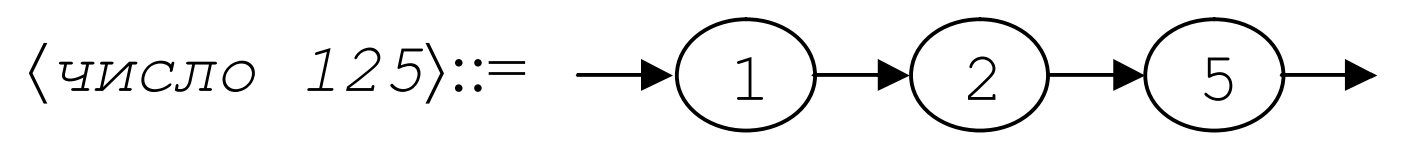
\includegraphics[width=0.65\textwidth]{pics/sdseq.png}  \\~\\     \pause
  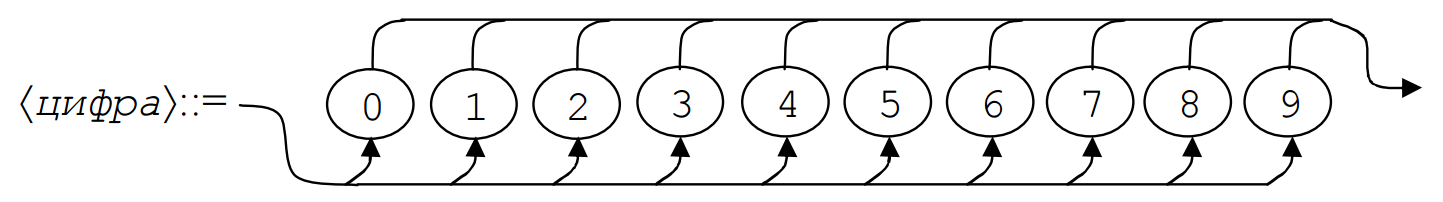
\includegraphics[width=1.0\textwidth]{pics/sddig.png}  \\~\\  \pause   
  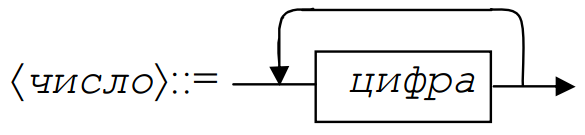
\includegraphics[width=0.45\textwidth]{pics/sdnum.png}  
\end{center}
\end{frame}


\begin{frame}[fragile]
  \transwipe[direction=90]
  \frametitle{Синтаксические диаграммы Вирта}
\begin{center}
  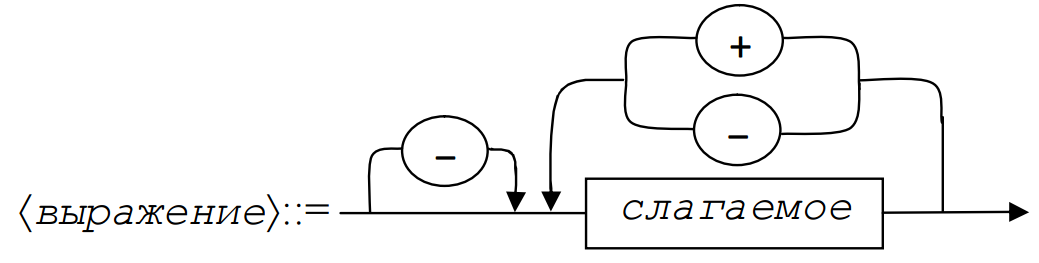
\includegraphics[width=0.75\textwidth]{pics/sdexpr.png}  \\~\\     \pause
  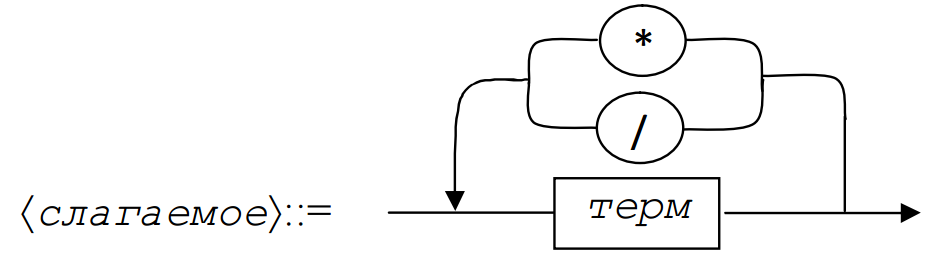
\includegraphics[width=0.75\textwidth]{pics/sdfact.png}  \\~\\  \pause   
  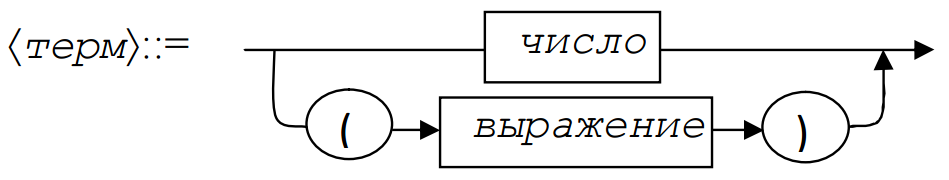
\includegraphics[width=0.75\textwidth]{pics/sdterm.png}  
\end{center}
\end{frame}

\begin{frame}[fragile]
  \transwipe[direction=90]
  \frametitle{Операции над строками}
  \begin{itemize}
    \item \textbf{Обращение (реверс) цепочки $a^R$} --- цепочка, символы которой записаны в обратном порядке
    \begin{itemize}
      \item Если $x = abc$, $x^R = cba$
      \item $\varepsilon^R = \varepsilon$
    \end{itemize}
    \item \textbf{$n-$я степень цепочки $a^n$} --- конкатенация $n$ повторений цепочки
    \begin{itemize}
      \item $a^0 = \varepsilon$
      \item $a^n = a \cdot a^{n-1} = a^{n-1} \cdot a$
    \end{itemize}
    \item \textbf{Длина цепочки $|a|$} --- количество составляющих ее символов
    \begin{itemize}
      \item $|babb| = 4, |babb|_a = 1, |babb|_b = 3, |babb|_c = 0$
      \item $|\varepsilon| = 0$
    \end{itemize}
  \end{itemize}
\end{frame}

\begin{frame}[fragile]
  \transwipe[direction=90]
  \frametitle{Формальный язык}
  \begin{itemize}
    \item $V$ --- алфавит
    \begin{itemize}
      \item $V = \{ 0, 1 \}$
    \end{itemize}
    \item $V^*$ --- множество, содержащее все цепочки в алфавите V, включая пустую цепочку
    \begin{itemize}
      \item $V^*=  \{ \varepsilon, 0, 1, 00, 11, 01, 10, 000, 001, 011, ... \}$
    \end{itemize}
    \item $V^+ = V^* \setminus \{ \varepsilon \} $ 
    \begin{itemize}
      \item $V^+ = \{0, 1, 00, 11, 01, 10, 000, 001, 011, \dots \}$
    \end{itemize}
    \item $Язык в алфавите V$ --- подмножество множества всех цепочек в этом алфавите. 
    \begin{itemize} 
      \item Для любого языка $L$ справедливо $L \in V^*$
    \end{itemize}
  \end{itemize}
\end{frame}

\begin{frame}[fragile]
  \transwipe[direction=90]
  \frametitle{Описание языка: формальная грамматика}
  \begin{itemize}
    \item \textbf{Порождающая грамматика $G$} --- это четверка $\langle V_T, V_N, P, S \rangle$

   \begin{itemize}
     \item $V_T$ --- алфавит терминальных символов (терминалов) 
     \item $V_N$ --- алфавит нетерминальных символов (нетерминалов)
     \begin{itemize} 
        \item $V_T \cap V_N = \emptyset$ 
        \item $V ::= V_T \cup V_N$
     \end{itemize}
     \item P --- конечное множество правил вида $\alpha \rightarrow \beta$
     \begin{itemize}
       \item $\alpha \in V^* V_N V^*$
       \item $\beta \in V^*$
     \end{itemize}  
     \item S --- начальный нетерминал грамматики, $S  \in N$
  \end{itemize}
  \end{itemize}
\end{frame}

\begin{frame}[fragile]
  \transwipe[direction=90]
  \frametitle{Пример: язык чисел в двоичной системе счисления}
$V_T = \{ 0, 1 \}; V_N = \{ S, N, A \}$

\begin{tabular}{p{3cm}  p{4cm}  p{3cm}}

$$
\begin{array}{crcl}
&S& \rightarrow & 0 \\
&S& \rightarrow & N \\
&S& \rightarrow & - N \\
&N& \rightarrow & 1 A \\
&A& \rightarrow & 0 A \\
&A& \rightarrow & 1 A \\
&A& \rightarrow & \varepsilon \\
\end{array}
$$

& \pause

$$
\begin{array}{crcl}
&S& \rightarrow & 0 \, | \, N \, | \, - N  \\
&N& \rightarrow & 1 A \\
&A& \rightarrow & 0 A \, | \, 1 A  \, | \, \varepsilon\\
\end{array}
$$

& \pause

$$
\begin{array}{crcl}
&S& \rightarrow & 0 \, | \, [-] N  \\
&N& \rightarrow & 1 A \\
&A& \rightarrow & (0 \, | \, 1) A  \, | \, \varepsilon\\
\end{array}
$$

\end{tabular}
\end{frame}

\begin{frame}[fragile]
  \transwipe[direction=90]
  \frametitle{Отношение непосредственной выводимости}
  \begin{itemize}
    \item $\alpha \rightarrow \beta \in P$
    \item $\gamma, \delta \in V^*$
    \item $\gamma \alpha \delta \Rightarrow \gamma \beta \delta$: $\gamma \beta \delta$ \textbf{непосредственно выводится} из $\gamma \alpha \delta$ при помощи правила $\alpha \rightarrow \beta$
  \end{itemize}
\end{frame}

\begin{frame}[fragile]
  \transwipe[direction=90]
  \frametitle{Отношение выводимости}
  \begin{itemize}
    \item $a_0, a_1, a_2, \dots, a_n \in V^*$
    \item $a_0 \Rightarrow a_1 \Rightarrow a_2 \Rightarrow \dots \Rightarrow a_n$
    \item $a_0 \xRightarrow[]{*} a_n$: $a_n$ \textbf{выводится} из $a_0$
  \end{itemize}

  \begin{itemize}
    \item $S \Rightarrow - N \Rightarrow - 1 A \Rightarrow - 1 1 A \xRightarrow[]{*} - 1 1 0 1 A \Rightarrow - 1 1 0 1$
  \end{itemize}
 \pause
  \begin{itemize}
    \item $\forall a \in V^*.a \xRightarrow[]{*} a$
  \end{itemize}

  \begin{itemize}
    \item $a_0 \xRightarrow[]{+} a_n$: вывод использует хотя бы одно правило грамматики
    \item $a_0 \xRightarrow[]{k} a_n$: вывод происходит за $k$ шагов
  \end{itemize}
\end{frame}


\begin{frame}[fragile]
  \transwipe[direction=90]
  \frametitle{Язык, порождаемый грамматикой $G = \langle V_T, V_N, P, S \rangle$}
  \begin{itemize}
    \item $L(G) = \{ \omega \in V_T^* \, | \, S \xRightarrow[]{*} \omega \}$
  \end{itemize}
\end{frame}

\begin{frame}[fragile]
  \transwipe[direction=90]
  \frametitle{Эквивалентность грамматик}
  \begin{itemize}
    \item Грамматики $G_1$ и $G_2$ \textbf{эквивалентны}, если $L(G_1) = L(G_2)$ \pause
  \end{itemize}
  
\begin{tabular}{p{6cm}  p{6cm}}

$$
\begin{array}{crcl}
&V_T &=& \{ 0, 1 \} \\
&V_N &=& \{ S, N, A \} \\~\\
&S& \rightarrow & 0 \, | \, N \, | \, - N  \\
&N& \rightarrow & 1 A \\
&A& \rightarrow & 0 A \, | \, 1 A  \, | \, \varepsilon\\
\end{array}
$$

& \pause

$$
\begin{array}{crcl}
&V_T &=& \{ 0, 1 \} \\
&V_N &=& \{ S, A \} \\~\\
&S& \rightarrow & 0 \, | \, 1 A  \, | \, - 1 A  \\
&A& \rightarrow &  0 A \, | \, 1 A  \, | \, \varepsilon\\
\end{array}
$$

\end{tabular}  
  
\end{frame}

\begin{frame}[fragile]
  \transwipe[direction=90]
  \frametitle{Контекстно-свободная грамматика}
  \begin{itemize}
    \item \textbf{Контекстно-свободная грамматика} --- грамматика, все правила которой имеют вид $A \rightarrow \alpha, A \in V_N, \alpha \in V^*$
  \end{itemize}
\end{frame}

\begin{frame}[fragile]
  \transwipe[direction=90]
  \frametitle{Дерево вывода}
  
  Дерево является \textbf{деревом вывода} для $G = \langle V_N, V_T, P, S\rangle$, если:  
  \begin{itemize}
    \item Каждый узел помечен символом из алфавита $V$
    \item Метка корня --- $S$
    \item Листья помечены терминалами, остальные узлы --- нетерминалами
    \item Если узлы $n_0, \dots, n_k$ --- прямые потомки узла $n$, перечисленные слева направо, с метками $A_0, \dots, A_k$; метка $n$ --- $A$, то $A \rightarrow A_0 \dots A_k \in P$
  \end{itemize}
\end{frame}

\begin{frame}[fragile]
  \transwipe[direction=90]
  \frametitle{Пример дерева вывода}
\begin{centering}

$G = \langle \{ S, A \}, \{ a, b \}, \{ S \rightarrow a A S | a, A \rightarrow S b A | b a | SS \}, S\rangle$  

$S \Rightarrow aAS \Rightarrow a S b A S \Rightarrow a a b A S \Rightarrow a a b b a S \Rightarrow a a b b a a$
    
  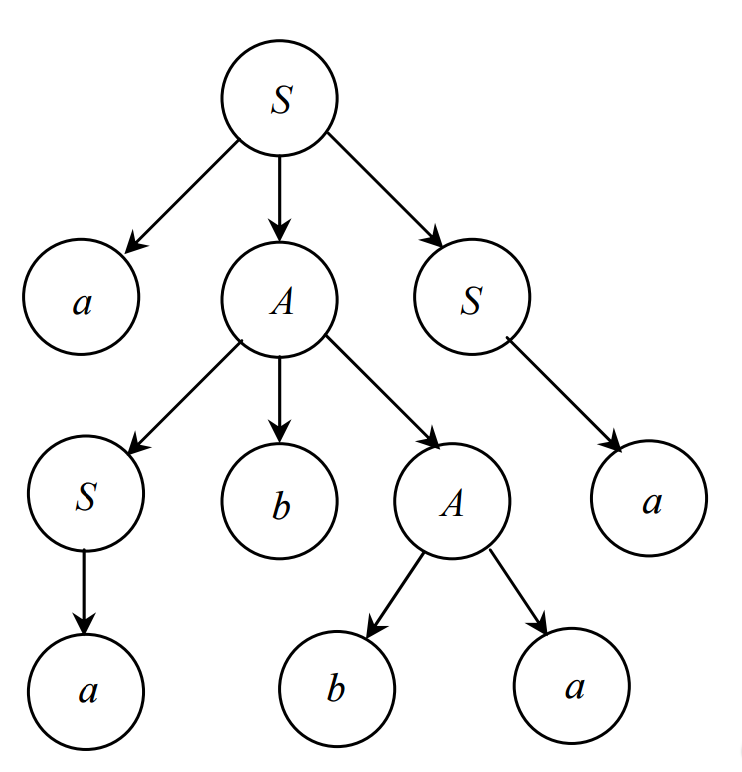
\includegraphics[width=0.55\textwidth]{pics/tree.png}  \\~\\     \pause

\end{centering}
\end{frame}

\begin{frame}[fragile]
  \transwipe[direction=90]
  \frametitle{Вывод и дерево вывода}
  \begin{rutheorem}[]
    Пусть $G = \langle V_N, V_T, P, S \rangle$ --- КС-грамматика
    
    Вывод $S \xRightarrow[]{*} \alpha$, где $\alpha \in V^*, \alpha \neq \varepsilon$ существует $\Leftrightarrow$ существует дерево вывода в грамматике G с результатом $\alpha$
  \end{rutheorem}

\end{frame}

\end{document}
